\documentclass{article}
\usepackage[utf8]{inputenc}
\usepackage[cyr]{aeguill}
\usepackage[francais]{babel}
\usepackage{graphicx}
\usepackage{amsmath}


\title{Reconnaissance des espèces de plantes grâce à la forme de leurs feuilles}

\author{Marie Lavigne, Thibaud Levasseur, Nicolas Monet}

\begin{document}
\maketitle
\newpage
\tableofcontents
\newpage
\section{Introduction}
Actuellement le nombre d'espèces de plantes sur Terre est estimé à 310 000 - 420 000, dont beaucoup encore inconnues. Leur reconnaissance a toujours été un enjeu primordial pour les populations, tant pour leur survie par la reconnaissance des plantes comestibles ou empoisonnées, que pour la protection de l'environnement. \\
Différentes méthodes furent utilisées pour les classifier, allant de la morphologie à l'étude cellulaire en passant par la phytochimie. Cependant, les avancées technologiques des dernières décennies en informatique et notamment dans le domaine de la vision nous permettent à présent d'utiliser les ordinateurs pour de telles classifications. \\
\\
Dans ce cas, quelle partie de la plante demander à l'algorithme de reconnaître ?
Les fleurs ? Disponibles uniquement lors des floraisons, elles forment pour un ordinateur un objet complexe puisqu'en 3D et dont une simple photo ne saurait capter l'intégralité des singularités qui les composent. Ainsi les fleurs seraient trop complexes à traiter pour un temps de présence trop court. 
Le même raisonnement peut être tenu pour les fruit et l'écorce quant à elle n'est disponible que sur trop peu de spécimens. \\
Reste alors les feuilles, présentes chez la majorité des plantes et durant une période plus longue que les fleurs puisqu'elles ne disparaissent habituellement qu'en hiver. Les feuilles ont la particularité d'être presque toujours en 2D permettant, à l'aide d'une simple photo du dessus, un traitement très simple de ses spécificités. \\
\\
Maintenant que le sujet d'étude est défini, nous devons penser aux critères de reconnaissance d'une espèce. En imagerie, deux critères principaux peuvent nous venir en tête pour différencier des feuilles : la couleur et la forme. \\
Cependant, la couleur d'une feuille peut énormément varier, que ce soit en fonction du changement de saison qu'à cause de l'ensoleillement ou de l'humidité. Ce critère n'est donc pas assez fiable pour être utilisé parallèlement à la forme. Ainsi, les images utilisées ne nécessiteront que des nuances de gris. \\
L'objet de notre étude portera en conclusion principalement sur les formes de feuilles variés que possèdent chaque plante.
\paragraph{}
Ce projet a été réalisé grâce au travail des chercheurs Ji-Xiang Du, Xiao-Feng Wang et Guo-Jun Zang et notamment à leur article publié sur science-direct.com ( 185 (2007) 883–93). Les données utilisées sont quant à elles issues du site internet http://archive.ics.uci.edu/ml/datasets.html.
\newpage

\section{Description des données}
Le jeu de donné utilisé comporte 360 feuilles en images couleur et noir et blanc réparties et triées en 36 espèces. Le nombres d'individu par groupe est assez réduit et ne dépasse pas le nombre de 16. Une imprécision peut donc apparaitre dû au nombre réduit d'individu dans chaque échantillon.
\paragraph{}
Les images ont une résolution de 960*720 pixel, ce qui offre précision suffisante, sans être excessive. Cependant le temps de calcul pour la sérialisation des données reste assez long : quelques secondes par image. Une sauvegarde de celle-ci est donc fortement conseillée.
\paragraph{}
La représentation des feuilles est homogène : l'image est centrée et pour chaque feuille le pétiole est placé vers le bas de l'image, ce qui permet de faciliter grandement le traitement de l'image dans la mesure ou aucune rotation n'est nécessaire en pré-traitement.

\begin{center}
	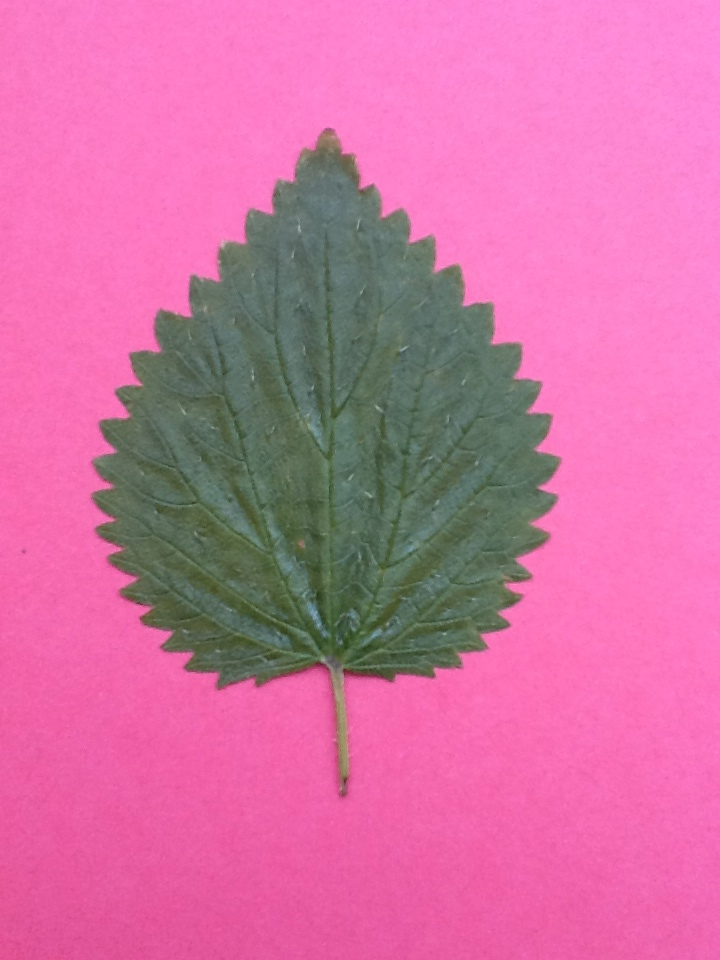
\includegraphics[scale=0.11]{image/urticaRGB.png}	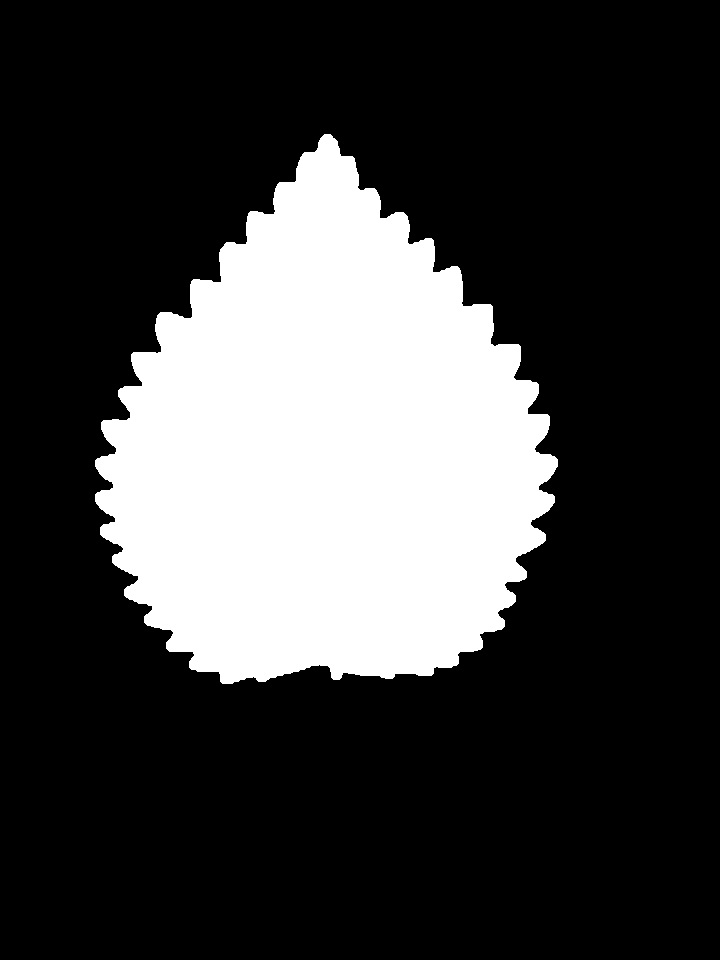
\includegraphics[scale=0.15]{image/urticaNB.png}
\end{center}
\section{Traitement des données}
\subsection{Définitions des propriétés géométriques invariantes}


Afin de séparer nos données, il est nécessaire de trouver les propriétés géométriques invariantes de chaque espèces de feuilles qui serviront à définir une hypersphères pour chaque espèce.

Afin de ne pas avoir de calculs trop lourds, nous avons faite le choix de nous limiter à une caractérisation de chaque feuille par un vecteur x $\in \Re ^{5}$. À ce vecteur sera ajouté un label pour l'apprentissage.

\subsubsection{Rectangularité}
La réctangularité est définie comme le rapport de la longueur sur la largeur du plus petit rectangle entourant la feuille.
\smallbreak
$R=\frac{longueur}{largeur}$
\subsubsection{Sphéricité}
La sphéricité est définie comme le rapport entre le rayon du cercle inscrit sur le rayon du cercle circonscrit.
\smallbreak
$S=\frac{r_{i}}{r_{c}}$
\subsubsection{Ratio d'aire}
Le ratio d'aire est le rapport entre l'air du polygone concave le plus petit circonscrit à la feuille et celle le plus petit rectangle entourant la feuille.
\smallbreak
$AO=\frac{A_{r}}{A_{C}}$
\subsubsection{Ratio de périmètre}
Le ratio de périmètre est le rapport entre le périmètre du polygone concave le plus petit circonscrit à la feuille et celui du plus petit rectangle entourant la feuille.
\smallbreak
$CP=\frac{P_{r}}{P_{C}}$
\subsubsection{Facteur de forme}
Le facteur de forme est une valeur utilisé pour décrire une feuille qui semble être empirique comme efficace. Elle est définit comme suit.
\smallbreak
$CP=\frac{4*\pi*R_{r}}{P_{r}^{2}}$
\subsection{Cas simple : deux espèces - Méthode de la séparation à vaste marge}
\subsubsection{Protocole}
Dans un premier temps nous avons cherché à résoudre le problème de façon simple, c'est à dire ne travailler que sur deux classes.
Suite à la définition de deux groupes de feuilles (ortie et érable dans notre exemple), il était possible de définir un hyperplan séparant ces deux groupes de feuilles grâce à la méthode de séparation à vaste marge.


\paragraph{}
Dans un premier temps, les feuilles sont étiquetées suivant leur classe par les valeurs \{ -1 ; 1 \}. 
\paragraph{}
On cherche ensuite une fonction telle que :
\smallbreak
 $\forall$x$\longrightarrow$f(x)$\in$\{ -1; 1 \}

\paragraph{}
L'identification de la feuille comme étant d'une espèce ou de l'autre correspond au résultat obtenu grâce à cette fonction.

\subsubsection{Résultats}
Les résultats obtenus lors de cette première série de test sont concluants dans la mesure où 100 \% des tests ont été fructueux. Cependant la petite taille de l'échantillon ne permet pas de réellement conclure sur la fiabilité des résultats même si ceux-ci sont plus que prometteurs.
\subsection{Cas général : plusieurs espèces - Méthode des K Plus Proches Voisins (K-nearest)}
\subsubsection{Protocole}
Pour rendre l'application plus utile, on veut pouvoir identifier une feuille directement, au lieu de seulement choisir si elle ressemble plus à une espèce ou à une autre.
On passe à quatre groupes de feuilles (ortie, érable, laurier et géranium dans notre exemple). On ne peut plus simplement séparer les classes par des hyperplans; on va plutot chercher à classifier les feuilles et à récupérer la classe la plus proche de notre feuille dans l'hyperplan.


\paragraph{}
Dans un premier temps, les feuilles sont étiquetées suivant leur classe par les un identifiant unique \{ 1 ; 2 ; 3 ; 4 \}. 
\paragraph{}
On repère dans l'hyperplan les coordonnées de la feuille à identifier.
\paragraph{}
On calcule la distance entre chaque point de l'hyperplan et le point de notre feuille. Ceci nous donne un vecteur de distances.
\paragraph{}
Enfin, on trie ce vecteur par ordre croissant de distances, et on décide que la classe de notre feuille est celle du premier point dans le vecteur, le point le plus proche.


\subsubsection{Résultats}
On obtient toujours 100 \% de succès sur nos tests avec quatre classes, pour un temps de calcul tout aussi négligeable que SVM. On peut donc affirmer qu'à petit volume, l'algorithme kppv est efficace et résoud notre problème de manière plus pertinente que SVM.

\newpage
\section{Conclusion}
Avec nos données de test (16 et 12 feuilles de 2 types différents) nous obtenons un taux de réussite de 100 \%.\\
Le temps d'apprentissage pour chaque image traité est d'environ une seconde. \\
Le temps d'exécution, quant à lui est autour d'une seconde, temps utilisé très majoritairement par la détermination des caractéristiques de la feuille. 
En conclusion nous pouvons dire que l'algorithme KPPV est rapide (et pourrait même l'être encore plus avec un appareil plus performant) mais aussi très efficace dans notre cas de test.
Il est cependant important de relativiser cette efficacité puisque nous avons sciemment choisi des feuilles de formes peu semblables. Il serait donc intéressant dans une extension de ce projet, de voir si des feuilles d'espèces de plantes différentes mais ayant des formes similaires auraient un taux de reconnaissance aussi élevé et si tel n'était pas le cas, quelles améliorations apportées.
\newpage
\section{Annexes}
Concernant le code: le programme utilise une fonction TIMVecteur qui renvoie un vecteur avec les caractéristiques de la feuille dans l'image passée en paramètre. Cette fonction est utilisée par le script createData, qui préalloue une matrice de taille fixe et arbitraire.
\smallbreak
Donc, si on modifie la taille du vecteur retourné par TIMVecteur, il faut modifier la ligne 4 de createData.m :
\begin{verbatim}
TIMVECTEUR_SIZE = 6;
\end{verbatim}
et changer 6 en la nouvelle taille de vecteur.

\paragraph{}
Le 5e élément du vecteur retourné par TIMVecteur vaut toujours 0. Ce paramètre correspond à la circularité, et causait des problèmes de calcul avec SVM. Nous avons donc omis ce paramètre.

\paragraph{}
Une amélioration possible (et probablement prioritaire) est la récupération automatique des données: pour l'instant, il faut spécifier à la main dans quels dossiers récupérer les données d'apprentissage, donner un label unique à chaque classe de données, et faire correspondre chaque label à un nom (fonction labelToName).
\smallbreak
A l'avenir il faudrait un dossier 'données' qui contiendrait un dossier par classe, et utiliser le nom de ces dossiers comme label pour nos données.

\end{document}
